\section{Análise e visualização}

\begin{frame}[fragile,t,label=cd-analise]{4. Agrupamento dos dados}
\texttt{groupby("curso")} separa a tabela por curso. Podemos calcular uma medida para cada grupo, ou várias com \texttt{agg()}.
\EMASCcodelabel{Notas disponíveis por curso}
\begin{lstlisting}
print(df_com_notas.groupby("curso")["nota"].median())
resumo = df_com_notas.groupby("curso")["nota"].agg(
    ["count", "mean", "median", "std", "min", "max"]
)
print(resumo.round(2))
print(df_com_notas.groupby("curso")["situacao"].value_counts())
\end{lstlisting}
\begin{EMASCnote}
\texttt{count} conta as notas disponíveis, \texttt{std} é o desvio padrão amostral e \texttt{value\_counts()} conta quantas notas há em cada categoria.
\end{EMASCnote}
\end{frame}

\begin{frame}[fragile,t]{4.1. Frequência relativa de notas ausentes}
Ao selecionar um registro ao acaso dentro de um curso, a probabilidade de sua nota estar ausente é:
\[
  P(\text{nota ausente}\mid\text{curso}) =
  \frac{\text{notas ausentes no curso}}{\text{registros no curso}}
\]
\EMASCcodelabel{Exemplo prático}
\begin{lstlisting}
cobertura = df.groupby("curso")["nota"].agg(["size", "count"])
cobertura["sem_nota"] = cobertura["size"] - cobertura["count"]
cobertura["pct_sem_nota"] = 100 * cobertura["sem_nota"] / cobertura["size"]
print(cobertura.round(2))
\end{lstlisting}
\begin{EMASCnote}
\texttt{size} conta todas as linhas e \texttt{count} ignora ausentes. Em Matemática, $1/6\approx 16{,}67\%$ (probabilidade condicional na base).
\end{EMASCnote}
\end{frame}

\begin{frame}[fragile,t]{5. Matplotlib / Gráfico de barras}
O gráfico de barras compara categorias: os cursos no eixo $x$ e o percentual de notas ausentes no eixo $y$.
\EMASCcodelabel{Percentual de notas ausentes por curso}
\begin{lstlisting}
plt.rcParams["font.size"] = 13   # Tamanho da fonte
plt.figure(figsize=(6, 4))       # Largura e altura
barras = plt.bar(cobertura.index, cobertura["pct_sem_nota"],
                 color="#358FD0")
plt.bar_label(barras, fmt="%.1f%%") # Valores nas barras
plt.title("Notas ausentes por curso")
plt.xlabel("Curso")
plt.ylabel("Notas ausentes (%)")
plt.ylim(0, 100)
plt.tight_layout()               # Ajusta o espaco
plt.show()                       # Exibe o grafico
\end{lstlisting}
\end{frame}

\begin{frame}[t]{5.1. Comparação dos cursos}
\begin{columns}[T,onlytextwidth]
\begin{column}{0.62\textwidth}
\centering
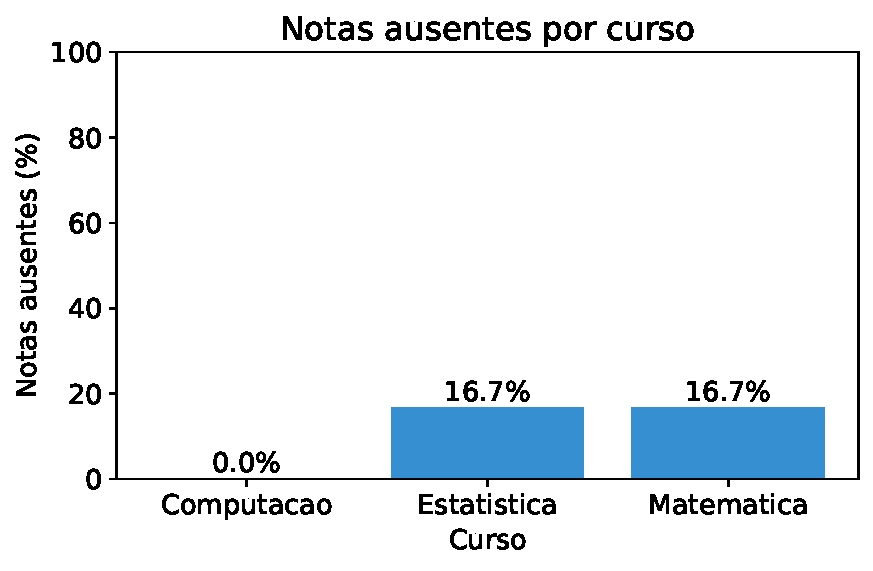
\includegraphics[width=\linewidth]{barras.pdf}
\end{column}
\begin{column}{0.35\textwidth}
\medskip
\textbf{Interpretação}
\begin{itemize}
  \item Matemática e Estatística: uma nota ausente em seis registros.
  \item Computação: todas as notas estão disponíveis.
\end{itemize}
\end{column}
\end{columns}
\end{frame}

\begin{frame}[fragile,t]{5.2. Histograma}
O histograma representa a distribuição de uma variável numérica. As barras mostram quantos valores pertencem a cada intervalo.
\EMASCcodelabel{Distribuição das notas disponíveis}
\begin{lstlisting}
plt.figure(figsize=(6, 4))
plt.hist(df_com_notas["nota"], bins=5, color="#358FD0", edgecolor="white")
plt.title("Distribuição das notas")
plt.xlabel("Nota")
plt.ylabel("Frequência absoluta")
plt.tight_layout()
plt.show()
\end{lstlisting}
\begin{EMASCnote}
\texttt{bins=5} define cinco intervalos de mesma largura entre a menor e a maior nota. As alturas são as contagens por intervalo.
\end{EMASCnote}
\end{frame}

\begin{frame}[t]{5.3. Distribuição das notas}
\begin{columns}[T,onlytextwidth]
\begin{column}{0.62\textwidth}
\centering
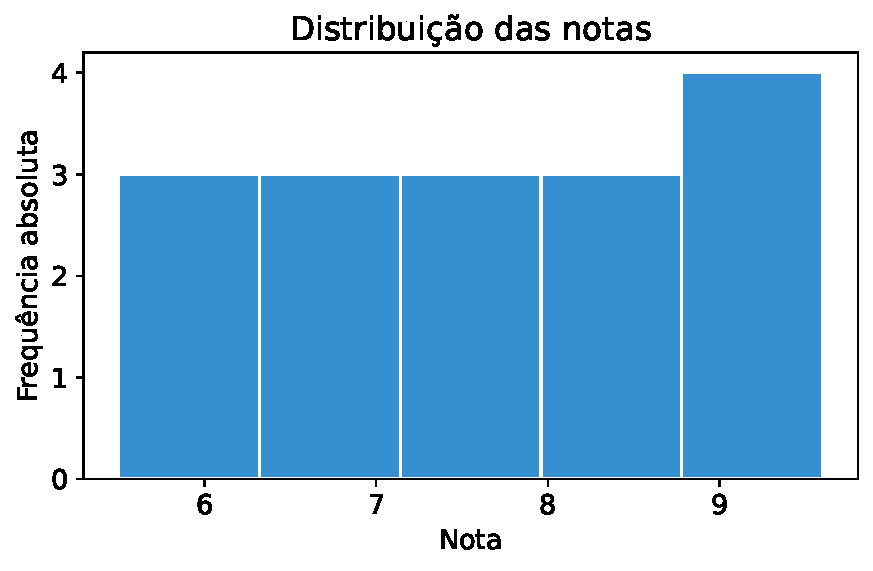
\includegraphics[width=\linewidth]{histograma.pdf}
\end{column}
\begin{column}{0.35\textwidth}
\medskip
\textbf{Interpretação}
\begin{itemize}
  \item As notas disponíveis variam de 5,5 a 9,6.
  \item Os quatro primeiros intervalos contêm três notas cada, e o último contém quatro.
\end{itemize}
\end{column}
\end{columns}
\end{frame}

\begin{frame}[fragile,t]{5.4. Gráfico de dispersão}
O gráfico de dispersão mostra a relação entre duas variáveis numéricas.
\EMASCcodelabel{Relação entre frequência e nota}
\begin{lstlisting}
plt.figure(figsize=(6, 4))
for curso, grupo in df_com_notas.groupby("curso"):
    plt.scatter(grupo["frequencia_pct"], grupo["nota"], label=curso)
plt.title("Frequência e nota")
plt.xlabel("Frequência (%)")
plt.ylabel("Nota")
plt.legend()
plt.tight_layout()
plt.show()
\end{lstlisting}
\begin{EMASCnote}
O laço separa os pontos por curso. \texttt{label} nomeia o grupo e \texttt{legend()} exibe a legenda.
\end{EMASCnote}
\end{frame}

\begin{frame}[t]{5.5. Relação entre frequência e nota}
\begin{columns}[T,onlytextwidth]
\begin{column}{0.62\textwidth}
\centering
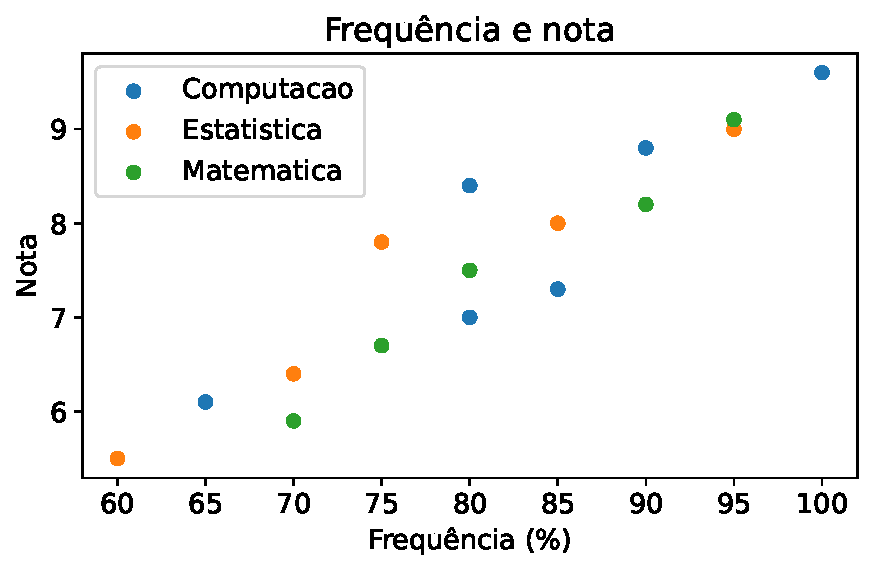
\includegraphics[width=\linewidth]{dispersao.pdf}
\end{column}
\begin{column}{0.35\textwidth}
\medskip
\textbf{Interpretação}
\begin{itemize}
  \item Nesta base, notas maiores tendem a acompanhar frequências mais altas.
  \item Essa associação, por si só, não demonstra uma relação de causa e efeito.
\end{itemize}
\end{column}
\end{columns}
\end{frame}
